
\begin{enumerate}
	\item Selecteer onder het File menu de optie Preferences.
	\item
		\begin{minipage}[t]{\linewidth}
		\raggedright
		\adjustbox{valign=t}{%
			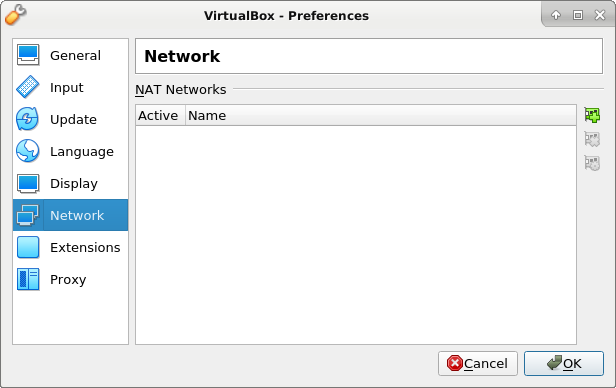
\includegraphics[width=0.99\linewidth]{linuxreader-img002.png}%
		}
		Click op het groene plusje aan de rechter kant.
		\end{minipage}

	\item
		\begin{minipage}[t]{\linewidth}
		\raggedright
		\adjustbox{valign=t}{%
			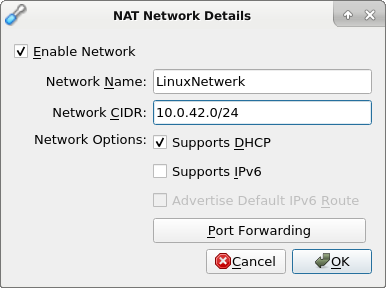
\includegraphics[width=0.99\linewidth]{linuxreader-img003.png}%
		}
		Geef het netwerk de naam ``LinuxNetwerk'' en een IP address range van 10.0.42.0. Click op OK om de wijzigingen op te slaan.
		\end{minipage}
\end{enumerate}

